\documentclass[12pt]{article}
\usepackage[dvips]{graphicx}
\topmargin -40pt
\headsep 30pt
\evensidemargin 0pt
\oddsidemargin 0pt
\textwidth 490pt
\textheight 650pt


\def\beq{\begin{equation}}
\def\eeq{\end{equation}}

\begin{document}

%\newpage
\section*{Verdict Quadrilateral Metrics:}

\subsection*{Variable Definitions:}

\begin{figure}[htb]
  \begin{center}
    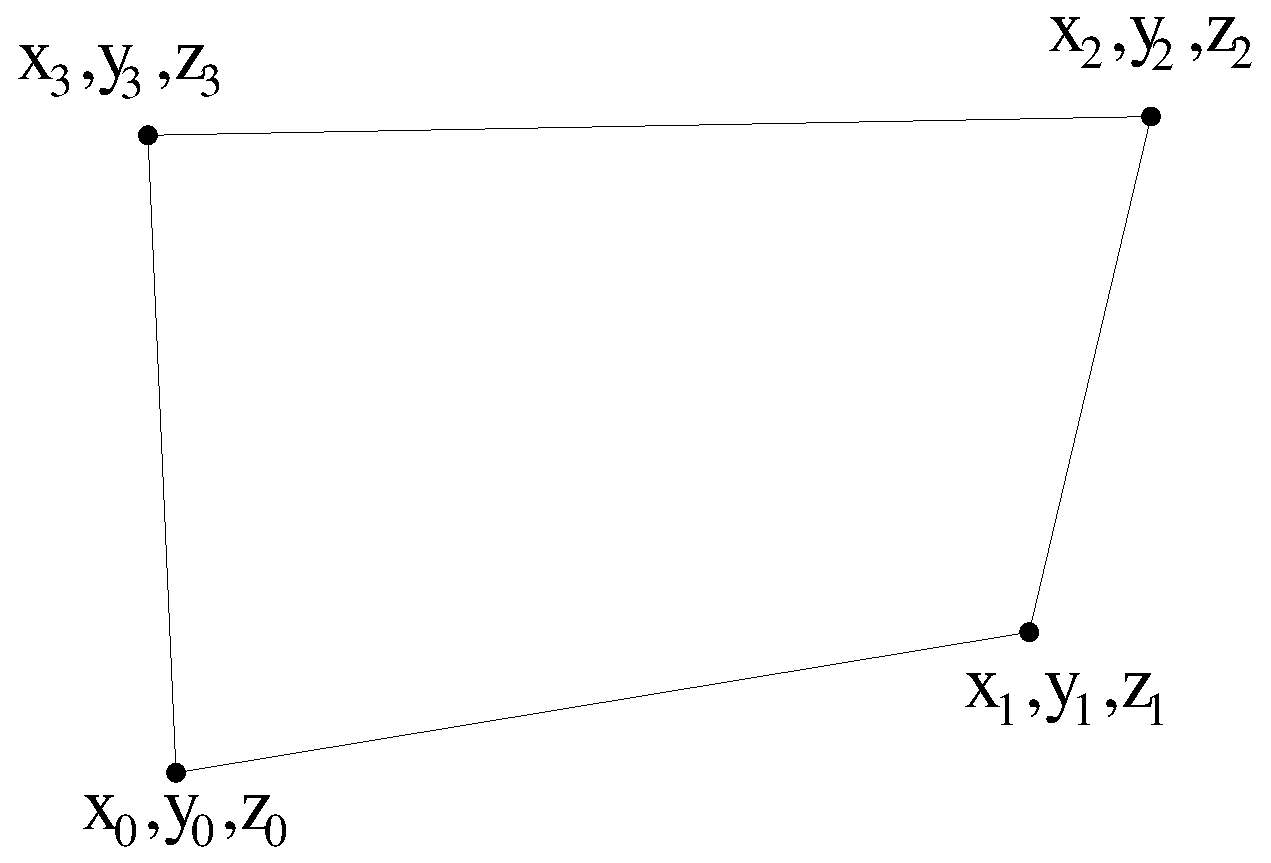
\includegraphics[height=2.0in]{quad.eps}
    \caption{Vertices of Quadrilateral}
    \label{fig:blank}
  \end{center}
\end{figure}

\subsubsection*{Quad Vertices:}
\begin{center}
$\vec P_0 = (x_0, y_0, z_0)$
\end{center}

\begin{center}
$\vec P_1 = (x_1, y_1, z_1)$
\end{center}

\begin{center}
$\vec P_2 = (x_2, y_2, z_2)$
\end{center}

\begin{center}
$\vec P_3 = (x_3, y_3, z_3)$
\end{center}

\subsubsection*{Quad Edge Vectors:}

\begin{center}
$\vec L_0 = \vec P_1 - \vec P_0 $
\end{center}

\begin{center}
$\vec L_1 = \vec P_2 - \vec P_1 $
\end{center}

\begin{center}
$\vec L_2 = \vec P_3 - \vec P_2 $
\end{center}

\begin{center}
$\vec L_3 = \vec P_0 - \vec P_3 $
\end{center}

\begin{center}
$L_{min} = MIN( |\vec L_0|,  |\vec L_1|, |\vec L_2|, |\vec L_3| ) $
\end{center}


\subsubsection*{Quad Diagonals:}

\begin{center}
$\vec D_0 = \vec P_2 - \vec P_0 $
\end{center}

\begin{center}
$\vec D_1 = \vec P_3 - \vec P_1 $
\end{center}

\begin{center}
$D_{max} = MAX( |\vec D_0|,  |\vec D_1| ) $
\end{center}

\subsubsection*{Principal Axes:}

\begin{center}
$\vec X_1 = \vec P_1 + \vec P_2 - \vec P_0 - \vec P_3 $
\end{center}

\begin{center}
$\vec X_2 = \vec P_2 + \vec P_3 - \vec P_0 - \vec P_1 $
\end{center}

\subsubsection*{Cross Derivative:}

\begin{center}
$\vec X_{12} = \vec P_0 + \vec P_2 - \vec P_1 - \vec P_3 $
\end{center}

\subsubsection*{Quad Corner Normals:}

\begin{center}
$\vec N_0 = \vec L_3 \times \vec L_0 $
\end{center}
\begin{center}
$\vec N_1 = \vec L_0 \times \vec L_1 $
\end{center}
\begin{center}
$\vec N_2 = \vec L_1 \times \vec L_2 $
\end{center}
\begin{center}
$\vec N_3 = \vec L_2 \times \vec L_3 $
\end{center}

\subsubsection*{Quad Corner Unit Normals:}

\begin{displaymath}
\hat n_0 = \frac{\vec N_0}{| \vec N_0 |} \,, 
\hat n_1 = \frac{\vec N_1}{| \vec N_1 |} \,,
\hat n_2 = \frac{\vec N_2}{| \vec N_2 |} \,,
\hat n_3 = \frac{\vec N_3}{| \vec N_3 |} 
\end{displaymath}

\subsubsection*{Quad Center Normal:}

\begin{center}
$ \vec N_{c} = \vec X_1 \times \vec X_2 $
\end{center}

\subsubsection*{Quad Center Unit Normal:}

\begin{displaymath}
\hat n_{c} = \frac{\vec N_{c}}{| \vec N_{c} |}
\end{displaymath}

\subsubsection*{Signed Corner Areas:}

For $k=0,1,2,3$, define

\begin{displaymath}
\alpha_k = \hat n_c \cdot \vec N_k 
\end{displaymath}

\noindent Note: if $\vec N_c = \vec 0$, then the signed corner areas are undefined, \newline
and all the metrics which depend on $\alpha_k$ are undefined. \newline
In this case, we set $\alpha_k = 0$ for $k=0,1,2,3$.

\subsection*{Overflow:}

\begin{flushleft}
NOTE:  The metrics below are all checked for overflow like so:
\end{flushleft}

\begin{flushleft}
${IF \quad metric\_value > 0;  \quad metric\_value = MIN( metric\_value, DBL\_MAX )}$
\end{flushleft}
 
\begin{flushleft}
${ELSE \quad metric\_value = MAX( metric\_value, -DBL\_MAX )}$
\end{flushleft}

\subsection*{Metric Ranges:}

\begin{flushleft}
Acceptable Range: Well-behaved elements will have metrics in this range.
\end{flushleft}
\begin{flushleft}
Normal Range:     All elements except those with degeneracies will have  \newline
                  metrics in this range.
\end{flushleft}
\begin{flushleft}
Full Range:       All elements including degenerate ones will have metrics \newline
                  in this range. 
\end{flushleft}


%---------------------------Area-----------------------------
\subsection*{Quad Area:}

\begin{displaymath}
area = \frac {1} {4} ( \alpha_0 + \alpha_1 + \alpha_2 + \alpha_3 )
\end{displaymath}

\begin{tabular}{lll}
& Metric Description:  & Average signed corner area. \\ 
& Dimension:           & $L^2$                   \\ 
& Acceptable Range:    & 0 to $DBL\_MAX$ \\ 
& Normal Range:        & 0 to $DBL\_MAX$ \\ 
& Full Range:          & $-DBL\_MAX$ to $DBL\_MAX$                       \\ 
& Value on Unit Square:& 1 \\
& Reference:           &  This Document. \\
\end{tabular} 


%---------------------------Aspect Ratio-----------------------------
\subsection*{Quad Aspect Ratio:}

\begin{center}
$aspect = MAX \left(  \left| \vec X_1 \right| / \left| \vec X_2 \right|, 
                            \left| \vec X_2 \right| / \left| \vec X_1 \right| \right)  $
\end{center} 

\begin{tabular}{lll}
& Metric Description:  & Maximum ratio of principle axes length. \\
& Dimension:           & $L^0$              \\ 
& Acceptable Range:    & 1 to 1.3               \\ 
& Normal Range:        & 1 to $DBL\_MAX$                      \\ 
& Full Range:          & 1 to $DBL\_MAX$ \\ 
& Value on Unit Square:& 1 \\
& Note:                & If $|\vec X_1|$ or $|\vec X_2| < DBL\_MIN$, $aspect~ratio = DBL\_MAX$  \\
& Reference:           & Adapted from \cite{one} \\
 
\end{tabular} 

%---------------------------Condition-----------------------------
\subsection*{Quad Condition:}

\begin{displaymath}
condition = \frac{1}{2} MAX \left(  \frac {|\vec L_0|^2 + |\vec L_3|^2 } { \alpha_0 },
                        \frac {|\vec L_1|^2 + |\vec L_0|^2 } { \alpha_1 },
                        \frac {|\vec L_2|^2 + |\vec L_1|^2 } { \alpha_2 },
                        \frac {|\vec L_3|^2 + |\vec L_2|^2 } { \alpha_3 } 
                \right)
\end{displaymath}

\begin{tabular}{lll}
& Metric Description:  & One-half minimum condition number at 4 corners. \\
& Dimension:           & $L^0$  \\
& Acceptable Range:    & 1 to 4 \\ 
& Normal Range:        & 1 to $DBL\_MAX$ \\ 
& Full Range:          & 1 to $DBL\_MAX$ \\ 
& Value on Unit Square:& 1 \\
& Note:                & If $\alpha_i< DBL\_MIN$, $condition = DBL\_MAX$  \\
& Reference:           &  \cite{three} \\
\end{tabular} 

%---------------------------Distortion-----------------------------
\subsection*{Quad Distortion:}

\begin{displaymath}
distortion = \frac{ |J|*master\textrm{-}area } { true\textrm{-}area }  
\end{displaymath}

\begin{flushleft} Where, \end{flushleft}
$|J| = $ minimum determinant of the Jacobian computed over all gauss points  \newline
of the element.  The location of the Gauss points is not documented. \newline 
$master\textrm{-}area =$ area of the master quad, where the master quad's corner \newline
nodes are as follows: \newline

 $\vec P_0 = (-1, -1, 0)$, 
 $\vec P_1 = (1, -1, 0)$, 
 $\vec P_2 = (1, 1, 0)$, 
 $\vec P_3 = ( -1, 1, 0)$ \newline

\begin{tabular}{lll}
& Metric Description:  & Minimum Gauss Point Jacobian divided by quad \\
&                      & area, times master quad's area. \\ 
& Dimension:           & $L^0$              \\ 
& Acceptable Range:    & 0.5 to 1            \\ 
& Normal Range:        & 0 to 1        \\ 
& Full Range:          & $-DBL\_MAX$ to $DBL\_MAX$        \\ 
& Value on Unit Square:& 1 \\
& Note:                & This metric is currently unsupported. \\ 
& Reference:           &  Adapted from \cite{five} \\
\end{tabular} 


%---------------------------Jacobian-----------------------------
\subsection*{Quad Jacobian:}

\begin{displaymath}
jacobian = MIN \left( \alpha_0, \alpha_1, \alpha_2, \alpha_3 \right)
\end{displaymath}

\begin{tabular}{lll}
& Metric Description:  & Minimum signed corner area at 4 corners. \\
& Dimension:           & $L^2$  \\ 
& Acceptable Range:    & 0 to $DBL\_MAX$   \\ 
& Normal Range:        & 0 to $DBL\_MAX$   \\ 
& Full Range:          & $-DBL\_MAX$ to $DBL\_MAX$        \\ 
& Value on Unit Square:& 1 \\
& Reference:           &  \cite{three} \\
\end{tabular} 

%---------------------------Maximum Angle-----------------------------
\subsection*{Quad Maximum Angle:}

\begin{displaymath}
\theta_i = \arccos{ \left( - \frac {\vec L_{i} \cdot \vec L_{i+1} }
                                {| \vec L_{i} | | \vec L_{i+1} |} \right) } 
                                  \left( \frac {180} {\pi} \right) 
\end{displaymath}

Where i = 0,1,2,3 and $\vec L_4 = \vec L_0$.

\begin{displaymath}
\theta_{max} = MAX\left( \theta_0, \theta_1, \theta_2, \theta_3 \right) 
\end{displaymath}

If $\alpha_0 < 0$ or $\alpha_1 < 0$ or $\alpha_2 < 0$ or $\alpha_3 < 0$

\begin{displaymath}
\theta_{max} = 360 - \theta_{max} 
\end{displaymath}


\begin{tabular}{lll}
& Metric Description:  & Maximum included quad angle.  \\
& Dimension:           & degrees                   \\ 
& Acceptable Range:    & 90 to 135 \\ 
& Normal Range:        & 90 to 360 \\ 
& Full Range:          & 0 to 360 \\ 
& Value on Unit Square:& 90 \\
& Note:                & If $|\vec L_i| \leq DBL\_MIN$ or $|\vec L_{i+1}| \leq DBL\_MIN$, \\
&                      & Verdict returns $\theta_{max} = 0.0$\\ 
& Reference:           & Traditional \\
\end{tabular} 

%---------------------------Minimum Angle-----------------------------
\subsection*{Quad Minimum Angle:}

\begin{displaymath}
\theta_i = \arccos{ \left( - \frac {\vec L_{i} \cdot \vec L_{i+1} }
                                {| \vec L_{i} | | \vec L_{i+1} |} \right) } 
                                  \left( \frac {180} {\pi} \right) 
\end{displaymath}

Where i = 0,1,2,3 and $\vec L_4 = \vec L_0$.

\begin{displaymath}
\theta_{min} = MIN\left( \theta_0, \theta_1, \theta_2, \theta_3 \right) 
\end{displaymath}


\begin{tabular}{lll}
& Metric Description:  & Minimum included quad angle.  \\
& Dimension:           & degrees                   \\ 
& Acceptable Range:    & 45 to 90 \\ 
& Normal Range:        & 0 to 90 \\ 
& Full Range:          & 0 to 360 \\ 
& Value on Unit Square:& 90 \\
& Note:                & If $|\vec L_i| \leq DBL\_MIN$ or $|\vec L_{i+1}| \leq DBL\_MIN$, \\
&                      & Verdict returns $\theta_{max} = 360.0$\\ 
& Reference:           & Traditional \\
\end{tabular} 


%---------------------------Oddy-----------------------------
\subsection*{Quad Oddy:}

\begin{displaymath}
O_k = \frac{(| \vec L_k |^2 - | \vec L_{k+1} |^2)^2 + 4 (\vec L_k \cdot \vec L_{k+1})^2}{2 | \vec N_{k+1} |^2 }
\end{displaymath}

Where k = 0,1,2,3 and $\vec L_4 = \vec L_0$.

\begin{displaymath}
oddy =  MAX \left( O_0, O_1, O_2, O_3 \right)
\end{displaymath}

\begin{tabular}{lll}
& Metric Description:  & Maximum deviation of metric tensor at quad corners. \\
& Dimension:           & $L^0$              \\ 
& Acceptable Range:    & 0 to 0.5               \\ 
& Normal Range:        & 0 to $DBL\_MAX$ \\ 
& Full Range:          & 0 to $DBL\_MAX$ \\ 
& Value on Unit Square:& 0 \\
& Note:                & If $|\vec N_{k+1}|^2 < DBL\_MIN$, $oddy = DBL\_MAX$  \\
& Reference:           &  Adapted from \cite{six} \\
\end{tabular} 


%---------------------------Relative Size-----------------------------
\subsection*{Quad Relative Size-Squared:}


\begin{displaymath}
R = \frac{Quad Area } {Average~Quad~Area}
\end{displaymath}

\begin{displaymath}
relative~size \textrm{-}squared =  [ MIN( R, \frac {1}{R}) ]^2
\end{displaymath}

\begin{flushleft}
$Average ~ Quad ~ Area$ is the average area of the quads in the \\
group of quads being analyzed. \\
\end{flushleft}

\begin{tabular}{lll}
& Metric Description:  & Square of minimum of the ratio of quad area to  \\
&                      & average quad area and the inverse ratio.\\
& Dimension:           & $L^0$  \\ 
& Acceptable Range:    & 0.3 to 1 \\ 
& Normal Range:        & 0 to 1 \\ 
& Full Range:          & 0 to 1 \\ 
& Value on Unit Square:& Depends on $Average ~ Quad ~ Area$ \\
& Note:                & If $Average~Quad~Area < DBL\_MIN; relative~size \textrm{-}squared = 0$ \\ 
&                      & If $R \leq DBL\_MIN; relative~size \textrm{-}squared = 0$ \\
& Reference:           &  \cite{four} \\
\end{tabular} 


%---------------------------Scaled Jacobian-----------------------------
\subsection*{Quad Scaled Jacobian:}

\begin{displaymath}
scaled~jacobian = MIN \left( \frac {\alpha_0} {|\vec L_0| |\vec L_3|}, 
                             \frac {\alpha_1} {|\vec L_1| |\vec L_0|},
                             \frac {\alpha_2} {|\vec L_2| |\vec L_1|},
                             \frac {\alpha_3} {|\vec L_3| |\vec L_2|} \right)
\end{displaymath}

\begin{tabular}{lll}
& Metric Description:  & Minimum Jacobian divided by the lengths of the 2 edge vectors, \\
&                      & (equals the minimum sine of the included angles). \\
& Dimension:           & $L^0$  \\ 
& Acceptable Range:    & 0.3 to 1 \\ 
& Normal Range:        & -1 to 1 \\ 
& Full Range:          & -1 to 1 \\ 
& Value on Unit Square:& 1 \\
& Note:                & If $L_{min} < DBL\_MIN$, $scaled~jacobian = 0$ \\
& Reference:           &  \cite{three} \\
\end{tabular} 

%---------------------------Shape-----------------------------
\subsection*{Quad Shape:}

\begin{displaymath}
shape = 2*MIN \left( \frac {\alpha_0} { |\vec L_0|^2 + |\vec L_3|^2 }, 
                     \frac {\alpha_1} { |\vec L_1|^2 + |\vec L_0|^2 }, 
                     \frac {\alpha_2} { |\vec L_2|^2 + |\vec L_1|^2 }, 
                     \frac {\alpha_3} { |\vec L_3|^2 + |\vec L_2|^2 }
\right) 
\end{displaymath}

\begin{tabular}{lll}
& Metric Description:  & 2/Condition number of Jacobian matrix. \\
& Dimension:           & $L^0$  \\ 
& Acceptable Range:    & 0.3 to 1 \\ 
& Normal Range:        & 0 to 1\\ 
& Full Range:          & 0 to 1\\ 
& Value on Unit Square:& 1 \\
& Note:                & If $\alpha_i < DBL\_MIN$, $shape = 0$ \\
&                      & If $L_{min} < DBL\_MIN$, $shape = 0$ \\
& Reference:           &  \cite{four} \\
\end{tabular} 


%---------------------------Shape and Size-----------------------------
\subsection*{Quad Shape and Size:}

\begin{displaymath}
shape~and~size = shape * relative~size \textrm{-}squared 
\end{displaymath}

\begin{tabular}{lll}
& Metric Description:  & Product of Shape and Relative Size.\\ 
& Dimension:           & $L^0$       \\ 
& Acceptable Range:    & 0.2 to 1 \\ 
& Normal Range:        & 0 to 1\\ 
& Full Range:          & 0 to 1\\ 
& Value on Unit Square:& 1 \\
& Reference:           & \cite{four} \\
\end{tabular} 



%---------------------------Shear-----------------------------
\subsection*{Quad Shear:}

\begin{displaymath}
shear = MIN \left( \frac {\alpha_0} {|\vec L_0| |\vec L_3|}, 
                             \frac {\alpha_1} {|\vec L_1| |\vec L_0|},
                             \frac {\alpha_2} {|\vec L_2| |\vec L_1|},
                             \frac {\alpha_3} {|\vec L_3| |\vec L_2|} \right)
\end{displaymath}

\begin{tabular}{lll}
& Metric Description:  & Same as scaled jacobian except for truncated range \\
& Dimension:           & $L^0$  \\ 
& Acceptable Range:    & 0.3 to 1 \\ 
& Normal Range:        & 0 to 1\\ 
& Full Range:          & 0 to 1\\ 
& Value on Unit Square:& 1 \\
& Note:                & If $\alpha_i < DBL\_MIN$, $shear = 0$ \\
&                      & If $L_{min} < DBL\_MIN$, $shear = 0$ \\
& Reference:           &  \cite{four} \\
\end{tabular} 

%---------------------------Shear and Size-----------------------------
\subsection*{Quad Shear and Size:}

\begin{displaymath}
shear~and~size = shear * relative~size \textrm{-}squared 
\end{displaymath}

\begin{tabular}{lll}
& Metric Description:  & Product of Shear and Relative Size-Squared.\\ 
& Dimension:           & $L^0$       \\ 
& Acceptable Range:    & 0.2 to 1 \\ 
& Normal Range:        & 0 to 1\\ 
& Full Range:          & 0 to 1\\ 
& Value on Unit Square:& 1 \\
& Reference:           & \cite{four} \\
\end{tabular} 


%---------------------------Skew-----------------------------
\subsection*{Quad Skew:}

\begin{displaymath}
\hat X_1 = \frac {\vec X_1} {| \vec X_1 |} 
\end{displaymath}

\begin{displaymath}
\hat X_2 = \frac {\vec X_2} {| \vec X_2 |} 
\end{displaymath}

\begin{displaymath}
skew = | \hat X_1 \cdot \hat X_2 |  
\end{displaymath}

\begin{tabular}{lll}
& Metric Description:  & $skew = |cos A|$, where $A$ is the angle between principle axes.\\
& Dimension:           & $L^0$              \\ 
& Acceptable Range:    & 0.5 to 1              \\ 
& Normal Range:        & 0 to 1\\ 
& Full Range:          & 0 to 1\\ 
& Value on Unit Square:& 1 \\
& Note:                & If $|\vec X_1|$ or $|\vec X_2| < DBL\_MIN$, $skew = 0$  \\
& Reference:           & Adapted from \cite{one} \\
 
\end{tabular} 

%---------------------------Stretch-----------------------------
\subsection*{Quad Stretch:}


\begin{displaymath}
stretch = \frac {\sqrt{ 2 } * L_{min}} 
                { D_{max} }
\end{displaymath}

\begin{tabular}{lll}
& Metric Description:  & $\sqrt{2}$ times the ratio of minimum edge length to \\
&                      & maximum diagonal. \\ 
& Dimension:           & $L^0$                   \\ 
& Acceptable Range:    & 0.25 to 1 \\
& Normal Range:        & 0 to 1 \\ 
& Full Range:          & 0 to $DBL\_MAX$ \\ 
& Value on Unit Square:& 1 \\ 
& Note:                & If $D_{max} < DBL\_MIN$, $stretch = DBL\_MAX$  \\
& Reference:           &  \cite{two} \\
\end{tabular} 


%---------------------------Taper-----------------------------
\subsection*{Quad Taper:}

\begin{displaymath}
taper = \frac {| \vec X_{12} |} {MIN \left( | \vec X_1 |, | \vec X_2 | \right)}
\end{displaymath}

\begin{tabular}{lll}
& Metric Description:  & Maximum ratio of cross derivative to minimum principle axes. \\ 
& Dimension:           & $L^0$              \\ 
& Acceptable Range:    & 0 to 0.7               \\ 
& Normal Range:        & 0 to $DBL\_MAX$ \\ 
& Full Range:          & 0 to $DBL\_MAX$ \\ 
& Value on Unit Square:& 0 \\
& Note:                & If $|\vec X_1|$ or $|\vec X_2| < DBL\_MIN$, $taper = DBL\_MAX$  \\
& Reference:           & Adapted from \cite{one} \\
 
\end{tabular} 


%---------------------------Warpage-----------------------------
\subsection*{Quad Warpage:}

\begin{displaymath}
warpage =  1 - MIN \left( 
    \left( \hat n_0 \cdot \hat n_2  \right) ^ 3
   ,\left( \hat n_1 \cdot \hat n_3  \right) ^ 3
         \right)
\end{displaymath}

\begin{tabular}{lll}
& Metric Description:  & Cosine of minimum dihedral angle formed by planes \\
&                      & intersecting in diagonals (to the fourth power). \\
& Dimension:           & $L^0$              \\ 
& Acceptable Range:    & 0 to 0.7        \\ 
& Normal Range:        & 0 to 2          \\ 
& Full Range:          & 0 to $DBL\_MAX$ \\ 
& Value on Unit Square:& 0 \\
& Note:                & If $|\vec N_k| < DBL\_MIN$ for any $k$, $warpage = DBL\_MAX$  \\
& Reference:           &  This Document \\
\end{tabular} 




\begin{thebibliography}{99}

\bibitem{one} J. Robinson, CRE Method of element 
testing and the Jacobian shape parameters, Eng. Comput., Vol 4, 1987.

\bibitem{two} FIMESH code.

\bibitem{three} P. Knupp, Achieving Finite Element Mesh Quality via 
Optimization of the Jacobian Matrix Norm and Associated Quantities,
Intl. J. Numer. Meth. Engng. 2000, 48:1165-1185.

\bibitem{four} P. Knupp, Algebraic Mesh Quality Metrics for Unstructured 
Initial Meshes, Finite Elements in Analysis and Design, Vol. 39, p217-241,
2003.

\bibitem{five} SDRC/IDEAS Simulation: Finite Element Modeling--User's Guide

\bibitem{six} A. Oddy, J. Goldak, M. McDill, and M. Bibby, ``A distortion 
metric for isoparametric finite elements,'' Trans. CSME, No. 38-CSME-32, 
Accession No. 2161, 1988.

\end{thebibliography}

\end{document}
